% !TeX root = enterprise-architecture-digital-blueprint.tex
% !TeX encoding = UTF-8
\chapter{Tata Kelola Arsitektur dan Praktik Arsitektur yang Lincah}

\section*{Tujuan Pembelajaran}
\begin{itemize}
  \item Merancang mekanisme tata kelola arsitektur: \textit{architecture board}, tinjauan kepatuhan, dispensasi, dan repositori.
  \item Membandingkan praktik EA (\textit{Enterprise Architecture}) tradisional dengan praktik yang lincah, termasuk tata kelola arsitektur di sektor publik.
  \item Mempresentasikan dan mempertahankan cetak biru transformasi digital di hadapan pemangku kepentingan.
\end{itemize}

\section{Pendahuluan}

Tiga belas bab sebelumnya menghasilkan cetak biru transformasi digital yang
utuh. Isinya visi arsitektur, potret kondisi saat ini, rancangan kondisi
target, \textit{gap analysis}, peta jalan 2026 sampai 2030, dan
\textit{business case}. Direksi menyetujuinya dalam satu rapat, lalu
dokumennya disimpan. Enam bulan kemudian, proyek-proyek berikutnya berjalan
tanpa pernah membukanya lagi.

Gejalanya mudah dikenali. Misalkan di Medikara Health, unit pemasaran membeli
aplikasi program loyalitas yang menyimpan data pasien sendiri. Rumah sakit
Bandung memperpanjang kontrak Sistem Informasi Manajemen Rumah Sakit (SIMRS)
versi lama tanpa klausul migrasi. Vendor Medikara+ menambah satu koneksi
langsung ke basis data SIMRS Depok karena itulah jalan tercepat. Tidak ada
yang berniat melanggar cetak biru. Masalahnya, tidak ada yang wajib bertanya,
dan tidak ada yang berwenang menjawab. Setahun kemudian, kondisi saat ini
justru lebih rumit daripada yang dipotret pada tonggak C2.

Bab ini membahas mekanisme yang membuat cetak biru tetap dipakai setelah
selesai disusun: tata kelola implementasi, manajemen perubahan arsitektur,
\textit{architecture board}, tinjauan kepatuhan, dispensasi, dan repositori
arsitektur. Pembahasannya mengikuti Fase G dan Fase H dalam Architecture
Development Method (ADM) serta bagian kemampuan dan tata kelola arsitektur
dalam The Open Group Architecture Framework (TOGAF) Standard \cite{togaf10}.
Tata kelola Sistem Pemerintahan Berbasis Elektronik (SPBE) dan Pemerintah
Digital dipakai sebagai pembanding \cite{perpres95-2018,perpres83-2025,permenpanrb8-2026}.
Open Agile Architecture Standard versi 2.0 \cite{oaa2} dipakai untuk menjaga
agar tata kelola tidak berubah menjadi birokrasi, dan temuan Lange dkk.
\cite{lange2016} dipakai untuk menilai apakah semua mekanisme itu memberi
nilai. Bab ini sekaligus menutup tonggak C4 dengan presentasi akhir cetak
biru.

\IfFileExists{../figures/ch14-diagram-konsep.png}{%

Gambar \ref{fig:ch14-ilustrasi-bab} merangkum hubungan komponen dan konsep utama bab ini.
\begin{figure}[!htb]
  \centering
  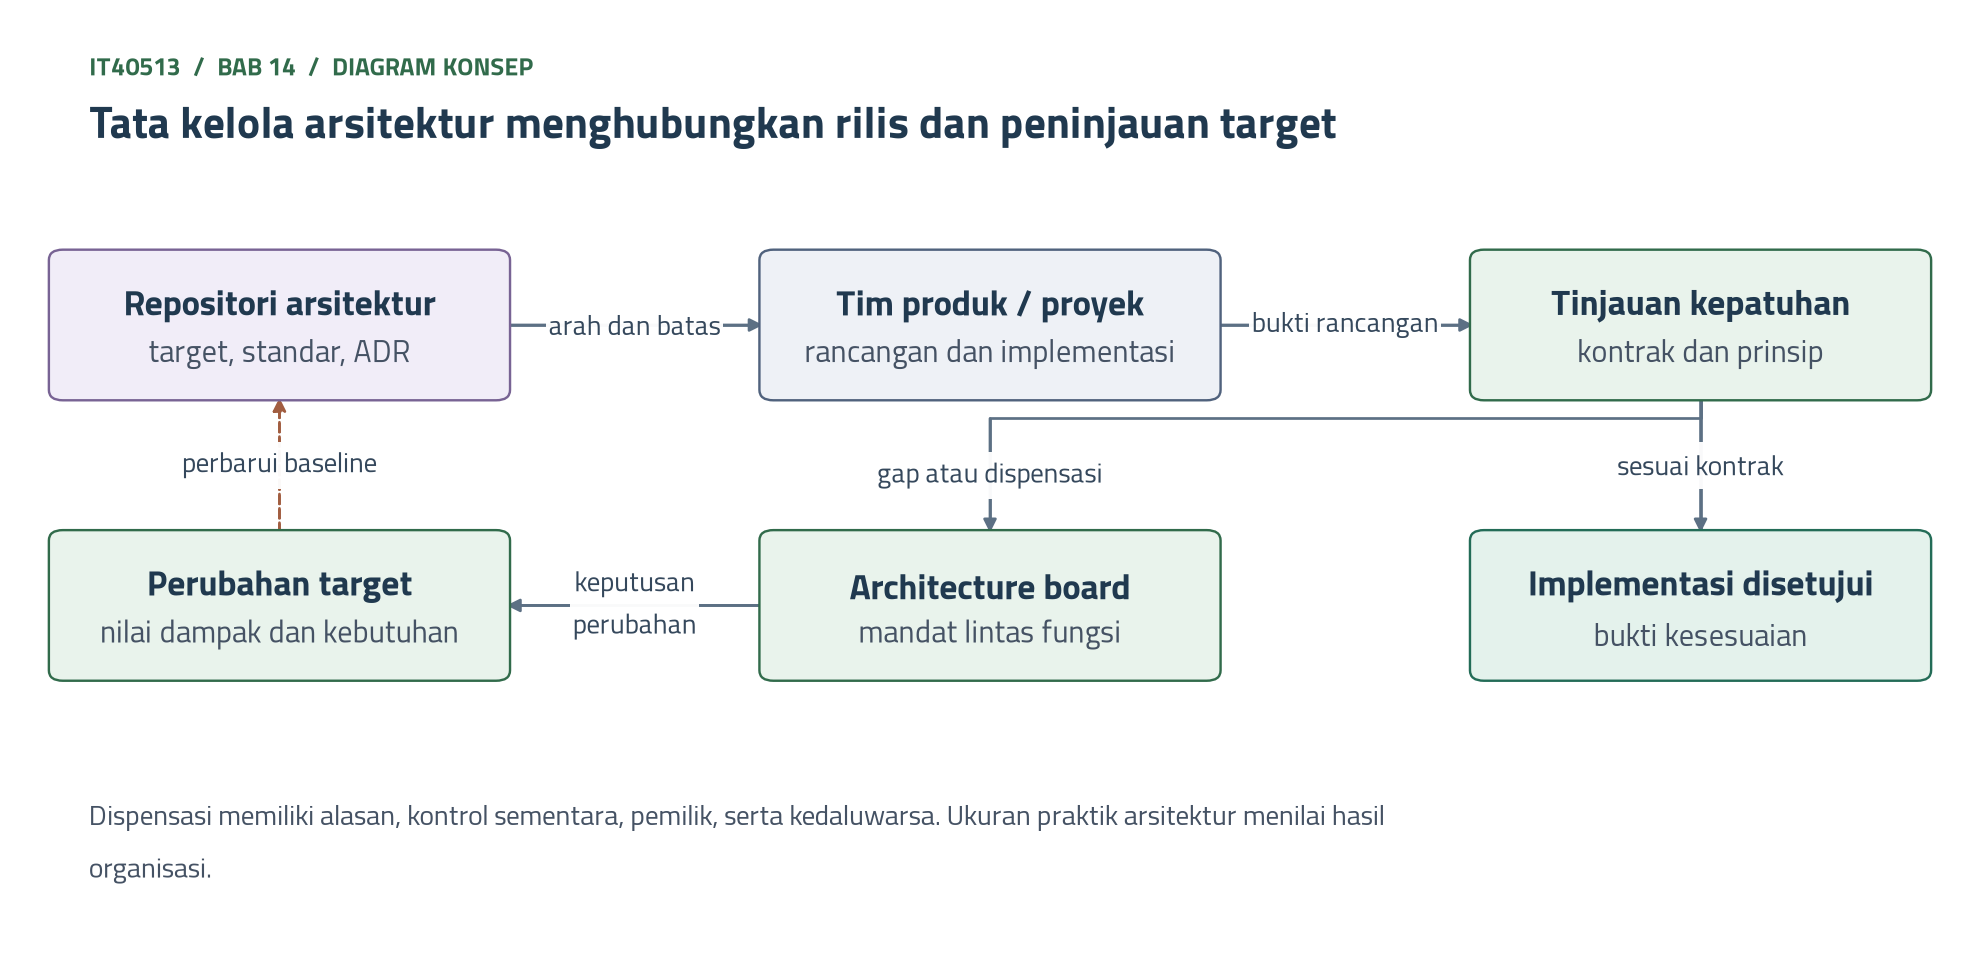
\includegraphics[width=\textwidth]{../figures/ch14-diagram-konsep.png}
  \caption{Tata kelola arsitektur menghubungkan rilis dan peninjauan target}
  \label{fig:ch14-ilustrasi-bab}
\end{figure}
}{}

\section{Tata Kelola Implementasi dan Manajemen Perubahan Arsitektur}

Peta jalan C4 berisi paket kerja yang akan dikerjakan banyak pihak: tim
teknologi informasi (TI) internal, vendor, dan mitra implementasi. Sebagian
besar orang di dalam tim itu tidak ikut menyusun cetak biru. Pertanyaan
pertama muncul: bagaimana memastikan hasil proyek mereka sesuai dengan
arsitektur target? Pertanyaan kedua menyusul: apa yang dilakukan bila
arsitektur target itu sendiri perlu berubah?

TOGAF menjawab kedua pertanyaan itu dengan dua fase terakhir ADM
\cite{togaf10}. Fase G, \textit{Implementation Governance}, memastikan setiap
proyek implementasi sesuai dengan arsitektur target. Alat utamanya adalah
kontrak arsitektur (\textit{architecture contract}) dan tinjauan kepatuhan.
Fase H, \textit{Architecture Change Management}, menjaga agar arsitektur
tetap relevan ketika bisnis, teknologi, dan regulasi berubah. Fase ini
menampung permintaan perubahan, menilai dampaknya, lalu memutuskan apakah
arsitektur cukup diperbarui atau perlu disusun ulang lewat siklus ADM yang
baru. Di tengah seluruh fase ada \textit{Requirements Management}, yaitu
proses yang mencatat dan menelusuri setiap kebutuhan sepanjang siklus.
Dengan proses ini, kebutuhan baru tidak langsung mengubah rancangan sebelum
dinilai.

Analoginya seperti membangun rumah dengan gambar arsitek. Kontraktor dan
tukang membangun, sedangkan konsultan pengawas memeriksa pada titik-titik
tertentu apakah pondasi, kolom, dan saluran air dikerjakan sesuai gambar
kerja. Bila pemilik rumah ingin menambah satu kamar, gambarnya diubah dan
disetujui lebih dahulu, bukan diputuskan tukang di lapangan. Konsultan
pengawas menjalankan peran Fase G, sedangkan prosedur perubahan gambar
menjalankan peran Fase H.

Gambar \ref{fig:ch14-siklus-gh} memperlihatkan hubungan kedua fase itu
dengan fase sebelumnya.

\begin{figure}[!htb]
  \centering
  \begin{tikzpicture}[
  font=\scriptsize,
  kotak/.style={draw, rounded corners, minimum height=0.95cm, text width=2.8cm,
                align=center, font=\scriptsize\bfseries},
  kecil/.style={draw, rounded corners, minimum height=0.7cm, text width=2.8cm,
                align=center, font=\scriptsize\bfseries},
  panah/.style={-{Stealth[length=2mm]}, thick}
]
  \node[kotak, fill=blue!8] (ef) at (0,0)
    {Fase E dan F\\{\tiny\mdseries peta jalan dan rencana migrasi}};
  \node[kotak, fill=orange!12] (g) at (4.3,0)
    {Fase G\\{\tiny\mdseries tata kelola implementasi: kontrak arsitektur dan tinjauan
    kepatuhan}};
  \node[kotak, fill=green!10] (hasil) at (8.6,0)
    {Solusi berjalan\\{\tiny\mdseries sesuai arsitektur target}};
  \node[kotak, fill=orange!12] (h) at (4.3,-3.0)
    {Fase H\\{\tiny\mdseries manajemen perubahan arsitektur}};
  \node[kotak, fill=praditagreen!15] (req) at (0,-3.0)
    {Requirements Management\\{\tiny\mdseries kebutuhan dicatat dan ditelusuri
    sepanjang siklus}};
  \node[kecil, fill=blue!8] (sederhana) at (8.6,-1.7)
    {Penyederhanaan\\{\tiny\mdseries manajemen perubahan biasa}};
  \node[kecil, fill=blue!8] (inkremental) at (8.6,-3.0)
    {Inkremental\\{\tiny\mdseries arsitektur diperbarui sebagian}};
  \node[kecil, fill=red!22] (ulang) at (8.6,-4.3)
    {Arsitektur ulang\\{\tiny\mdseries siklus ADM baru dari Fase A}};

  \draw[panah] (ef) -- (g);
  \draw[panah] (g) -- (hasil);
  \draw[panah] (g) -- (h);
  \draw[panah] (h.east) -- ++(0.55,0) |- (sederhana.west);
  \draw[panah] (h.east) -- (inkremental.west);
  \draw[panah] (h.east) -- ++(0.55,0) |- (ulang.west);
  \draw[dashed, thick, gray] (req) -- (h);
  \draw[dashed, thick, gray] (req) -- (ef);
  \draw[dashed, thick, gray] (req.north east) -- (g.south west);

  \node[font=\tiny, gray, anchor=west] at (4.4,-1.5) {permintaan perubahan};
  \node[font=\tiny, gray, align=center, anchor=north] at (4.3,-3.7)
    {pemicu: proyek, strategi bisnis,\\teknologi baru, dan regulasi};
\end{tikzpicture}

  \caption{Fase G mengawal proyek menuju arsitektur target, sedangkan Fase H
           memilah permintaan perubahan menurut besar dampaknya}
  \label{fig:ch14-siklus-gh}
\end{figure}

Kontrak arsitektur adalah kesepakatan tertulis antara fungsi arsitektur,
sponsor proyek, dan tim pelaksana tentang luaran, mutu, dan kesesuaian
solusi dengan arsitektur target \cite{togaf10}. Isinya umumnya empat hal:
ruang lingkup solusi, prinsip dan standar yang wajib dipenuhi, titik
tinjauan selama proyek berjalan, dan cara menangani penyimpangan. Kontrak
ditandatangani sebelum proyek mulai membangun, karena sesudah itu biaya
untuk berbalik arah naik setiap minggu.

Dua contoh dari Medikara:

\begin{enumerate}
  \item Misalkan proyek Master Patient Index (MPI) pada tahun pertama peta
        jalan mencantumkan tiga titik tinjauan dalam kontraknya: rancangan
        solusi, sebelum uji terima, dan sebelum dipakai di rumah sakit
        pertama. Pada tinjauan pertama, board menemukan bahwa rancangan
        vendor masih memakai nomor rekam medis tiap rumah sakit sebagai kunci
        utama. Perbaikannya cukup mengubah dokumen rancangan, karena belum
        ada kode yang ditulis.
  \item Misalkan proyek platform integrasi berjanji memindahkan 23 koneksi
        \textit{point-to-point} yang masih aktif ke platform bersama dalam
        dua tahun. Kontraknya memuat target antara: 8 koneksi pertama dalam
        12 bulan, dimulai dari koneksi ke Badan Penyelenggara Jaminan Sosial
        (BPJS) Kesehatan dan SATUSEHAT yang paling sering bermasalah.
        Tinjauan pada bulan ke-12 cukup menghitung koneksi yang benar-benar
        sudah pindah.
\end{enumerate}

\subsection*{Permintaan perubahan dan klasifikasinya}

Arsitektur target disusun berdasarkan keadaan pada saat penyusunannya, dan
keadaan itu terus bergeser. Pemicunya datang dari empat arah: proyek yang
menemukan kendala, strategi bisnis yang berubah, teknologi yang berganti
versi atau berhenti didukung vendor, dan regulasi baru. TOGAF membagi
perubahan menjadi tiga kelas menurut besar dampaknya, yaitu penyederhanaan,
inkremental, dan arsitektur ulang \cite{togaf10}. Tabel
\ref{tab:ch14-perubahan} memuat ketiganya beserta contoh di Medikara.

\begin{table}[!htb]
  \centering
  \caption{Tiga kelas perubahan arsitektur dan cara menanganinya}
  \label{tab:ch14-perubahan}
  \begin{tabularx}{\textwidth}{>{\raggedright\arraybackslash}p{2.9cm}>{\raggedright\arraybackslash}X>{\raggedright\arraybackslash}X}
    \hline
    \textbf{Kelas} & \textbf{Contoh di Medikara} & \textbf{Penanganan} \\
    \hline
    Penyederhanaan & Versi minimum PostgreSQL di katalog standar dinaikkan
      karena versi lama berhenti didukung & Manajemen perubahan biasa, lalu
      dicatat di repositori \\
    \hline
    Inkremental & Asuransi mitra baru memakai format klaim yang berbeda,
      sehingga arsitektur integrasi mitra perlu ditambah & Diperbarui
      sebagian lewat keputusan board, kadang dengan mengulang sebagian fase
      ADM \\
    \hline
    Arsitektur ulang & Misalkan Medikara mengakuisisi jaringan 25 klinik
      yang memakai sistem berbeda & Siklus ADM baru dimulai dari Fase A \\
    \hline
  \end{tabularx}
\end{table}

Dua hal pada perubahan sering tertukar. Pembagiannya begini. Manajemen
perubahan TI sehari-hari mengatur perubahan pada sistem yang sudah berjalan,
misalnya pemasangan \textit{patch}, perubahan konfigurasi, atau penambahan
kolom laporan. Manajemen perubahan arsitektur mengatur perubahan pada arah,
yaitu prinsip, standar, dan arsitektur target. Keduanya bersambung di satu
titik. Perubahan operasional yang ternyata menyentuh standar, misalnya
vendor ingin mengganti basis data sebuah aplikasi, dinaikkan dari manajemen
perubahan TI ke Fase H.

\textit{Requirements Management} menjaga sambungan itu. Misalkan BPJS
Kesehatan mengubah ketentuan teknis pengajuan klaim. Kebutuhan baru itu
dicatat di repositori kebutuhan, ditelusuri ke kapabilitas Pengelolaan
Klaim dan ke aplikasi yang terdampak, lalu dinilai kelasnya. Tanpa
pencatatan ini, kebutuhan regulator biasanya langsung dikerjakan vendor di
satu rumah sakit, dan empat rumah sakit lainnya menyusul dengan caranya
masing-masing. Hasilnya lima cara berbeda untuk satu kewajiban yang sama.

\section{Architecture Board dan Tinjauan Kepatuhan}

Kontrak dan tinjauan membutuhkan pihak yang berwenang memutuskan. Pertanyaan
kemudian muncul: siapa yang memutuskan bila sebuah proyek bertentangan
dengan prinsip arsitektur? Tanpa forum yang jelas, keputusan jatuh kepada
pihak yang suaranya paling keras atau tenggatnya paling dekat. Biasanya itu
berarti prinsip dikalahkan oleh tenggat.

\textit{Architecture board} adalah forum lintas fungsi yang diberi mandat
untuk mengambil keputusan arsitektur atas nama organisasi. Menurut TOGAF,
tanggung jawabnya meliputi menjaga konsistensi antarbagian arsitektur,
menegakkan kepatuhan, memutuskan dispensasi, menyetujui perubahan
arsitektur, dan mendorong pemakaian ulang komponen \cite{togaf10}. TOGAF
menyarankan board yang kecil, yaitu empat atau lima anggota tetap dan tidak
lebih dari sepuluh, agar keputusan tetap dapat diambil \cite{togaf10}.
Mandat board ditulis dalam piagam yang disahkan direksi. Tanpa pengesahan
itu, keputusan board hanya berupa saran.

Analoginya seperti pengurus RT yang memberi izin renovasi. Warga bebas
mengecat rumah atau mengganti lantai tanpa bertanya. Namun, menggeser
saluran air bersama atau menutup jalan kampung harus dibicarakan dengan
pengurus, karena dampaknya dirasakan tetangga. Board bekerja dengan logika
yang sama: keputusan yang hanya berdampak di dalam satu proyek diserahkan
kepada proyek, sedangkan keputusan yang menyentuh kepentingan bersama
dibawa ke board.

\subsection*{Keanggotaan dan pelibatan bisnis}

Board yang seluruh anggotanya orang TI mudah dipandang sebagai urusan
teknis. Survei SAP LeanIX terhadap 360 arsitek \textit{enterprise} menemukan
bahwa 92 persen responden menyatakan EA masih dipandang, seluruhnya atau
sebagian, sebagai fungsi administratif TI \cite{leanix2025}. Laporan yang
sama menyebut keikutsertaan pemangku kepentingan bisnis di dalam forum
tinjauan arsitektur sebagai langkah awal yang baik untuk mengubah pandangan
itu \cite{leanix2025}.

Misalkan Medikara menetapkan lima anggota tetap:

\begin{enumerate}
  \item Direktur Strategi dan Transformasi sebagai ketua, karena pemilik
        strategi ``Satu Pasien, Satu Rekam Medis'' harus ikut memutuskan.
  \item Direktur Pelayanan, yang mewakili dokter dan perawat sebagai
        pemakai sistem klinis.
  \item Direktur Keuangan, yang memegang ERP (\textit{Enterprise Resource
        Planning}) keuangan dan menanggung biaya integrasi.
  \item Kepala TI, yang menanggung operasi seluruh sistem.
  \item Kepala Arsitek \textit{Enterprise} sebagai sekretaris, yang
        menyiapkan bahan rapat dan menjaga repositori.
\end{enumerate}

Petugas pelindungan data, kepala keamanan informasi atau \textit{Chief
Information Security Officer} (CISO), dan direktur rumah sakit yang terdampak
hadir sebagai undangan sesuai agenda. Rapat rutin
digelar sebulan sekali selama dua jam. Board tidak memutuskan anggaran
proyek. Keputusan investasi tetap berada di komite pengarah TI dan direksi,
yang strukturnya dibahas rinci di IT40813.

\subsection*{Daftar periksa kepatuhan}

Tinjauan kepatuhan menilai apakah rancangan atau hasil proyek sesuai dengan
arsitektur. Supaya tinjauan tidak bergantung pada selera peninjau,
pertanyaannya diturunkan dari prinsip arsitektur yang sudah disepakati pada
tonggak C1. Setiap prinsip menghasilkan satu atau dua pertanyaan yang
jawabannya dapat dibuktikan, bukan sekadar diyakini. Tabel
\ref{tab:ch14-daftar-periksa} memperlihatkan contohnya untuk lima prinsip
tinjauan Medikara, dengan kode PT1 sampai PT5. Kelimanya rumusan operasional,
bukan pengganti enam prinsip PA1 sampai PA6 di Bab 3. PT1 menerjemahkan PA1
dan PA3, PT2 menerjemahkan PA2, PT3 menerjemahkan PA5, sedangkan PT4 dan PT5
ditambahkan untuk tinjauan ini. Baris PT3 memakai HL7 FHIR, yaitu standar pertukaran data
kesehatan Health Level Seven (HL7) Fast Healthcare Interoperability
Resources (FHIR) yang juga dipakai SATUSEHAT. Pemakaiannya dari sisi
integrasi dibahas rinci di IT40613.

\begin{table}[!htb]
  \centering
  \caption{Daftar periksa kepatuhan yang diturunkan dari lima prinsip
           tinjauan Medikara}
  \label{tab:ch14-daftar-periksa}
  \begin{tabularx}{\textwidth}{>{\raggedright\arraybackslash}p{2.3cm}>{\raggedright\arraybackslash}X>{\raggedright\arraybackslash}X}
    \hline
    \textbf{Prinsip} & \textbf{Pertanyaan periksa} & \textbf{Bukti yang diminta} \\
    \hline
    PT1 Satu sumber data pasien & Apakah identitas pasien diambil dari MPI,
      bukan dibuat sendiri oleh aplikasi? & Diagram aliran data dan daftar
      tabel yang menyimpan identitas pasien \\
    \hline
    PT2 Akses berbasis peran dan tercatat & Apakah pengguna masuk lewat
      layanan identitas terpusat, dan apakah setiap akses ke rekam medis
      tercatat? & Rancangan otentikasi dan contoh catatan akses \\
    \hline
    PT3 Integrasi lewat antarmuka standar & Apakah pertukaran data klinis
      memakai HL7 FHIR lewat platform integrasi? & Katalog antarmuka proyek \\
    \hline
    PT4 Utamakan layanan bersama & Apakah fungsi yang sama sudah disediakan
      layanan bersama yang ada? & Hasil penelusuran katalog aplikasi \\
    \hline
    PT5 Data pasien dilindungi sejak rancangan & Apakah data pasien hanya
      dikumpulkan seperlunya dan disimpan di lokasi yang diizinkan? &
      Penilaian dampak pelindungan data dan rancangan penyimpanan \\
    \hline
  \end{tabularx}
\end{table}

Hasil tinjauan dinyatakan dengan tingkat kepatuhan. TOGAF membedakan enam
tingkat, seperti pada Tabel \ref{tab:ch14-tingkat-kepatuhan}
\cite{togaf10}. Pembedaan ini berguna karena ``tidak patuh'' ternyata punya
beberapa bentuk yang akibatnya berbeda.

\begin{table}[!htb]
  \centering
  \caption{Enam tingkat kepatuhan menurut TOGAF beserta contoh di Medikara}
  \label{tab:ch14-tingkat-kepatuhan}
  \begin{tabularx}{\textwidth}{>{\raggedright\arraybackslash}p{2.2cm}>{\raggedright\arraybackslash}X>{\raggedright\arraybackslash}X}
    \hline
    \textbf{Tingkat} & \textbf{Artinya} & \textbf{Contoh} \\
    \hline
    Tidak relevan (\textit{irrelevant}) & Solusi tidak bersinggungan dengan
      spesifikasi arsitektur & Aplikasi jadwal piket satpam dinilai
      terhadap standar data klinis \\
    \hline
    Konsisten (\textit{consistent}) & Sebagian fitur sama dan dikerjakan
      sesuai spesifikasi, tetapi ada fitur spesifikasi yang belum dikerjakan
      dan ada fitur lain di luar spesifikasi & Sistem laboratorium mengirim
      hasil lewat FHIR, belum mencatat akses, dan menambah saluran pesan
      sendiri \\
    \hline
    Patuh (\textit{compliant}) & Sebagian spesifikasi belum dikerjakan,
      tetapi semua yang dikerjakan sesuai spesifikasi & Medikara+ versi baru
      memakai MPI untuk janji temu, sedangkan telekonsultasi belum dipindah \\
    \hline
    Sesuai (\textit{conformant}) & Seluruh spesifikasi dikerjakan, ditambah
      fitur lain yang tidak sesuai spesifikasi & Aplikasi memakai MPI
      sepenuhnya, tetapi juga menyalin data pasien ke \textit{spreadsheet}
      untuk laporan \\
    \hline
    Sesuai penuh (\textit{fully conformant}) & Spesifikasi dan solusi cocok
      sepenuhnya & Proyek MPI pada akhir uji terima \\
    \hline
    Tidak sesuai (\textit{non-conformant}) & Ada fitur spesifikasi yang
      dikerjakan secara bertentangan dengan spesifikasi & Aplikasi membuat
      nomor pasien sendiri walaupun spesifikasi mewajibkan MPI \\
    \hline
  \end{tabularx}
\end{table}

\subsection*{Dispensasi yang cepat tetapi terkendali}

Tidak semua penyimpangan dapat dihindari. Tenggat regulator, kontrak dengan
pelanggan, atau komponen pendukung yang belum siap kadang memaksa proyek
berjalan dengan solusi yang belum patuh. Dispensasi (\textit{dispensation})
adalah izin resmi untuk menyimpang dari arsitektur dalam waktu tertentu dan
dengan syarat tertentu. TOGAF menekankan bahwa dispensasi diberikan untuk
jangka waktu terbatas, dan sifat berbatas waktu itulah yang memicu tinjauan
kepatuhan berikutnya \cite{togaf10}. Gambar \ref{fig:ch14-alur-dispensasi}
memperlihatkan alur yang dipakai Medikara.

\begin{figure}[!htb]
  \centering
  \begin{tikzpicture}[
  font=\scriptsize,
  kotak/.style={draw, rounded corners, minimum height=0.95cm, text width=2.3cm,
                align=center, font=\scriptsize\bfseries},
  tanya/.style={draw, diamond, aspect=1.7, inner sep=1pt, align=center,
                font=\scriptsize\bfseries},
  panah/.style={-{Stealth[length=2mm]}, thick}
]
  \node[kotak, fill=blue!8] (rancangan) at (0,0)
    {Rancangan solusi\\{\tiny\mdseries diajukan tim proyek}};
  \node[kotak, fill=blue!8] (tinjau) at (3.1,0)
    {Tinjauan kepatuhan\\{\tiny\mdseries daftar periksa dari prinsip}};
  \node[tanya, fill=orange!12] (patuh) at (6.2,0) {Patuh?};
  \node[kotak, fill=green!10] (kontrak) at (9.3,0)
    {Kontrak arsitektur\\{\tiny\mdseries proyek lanjut}};
  \node[kotak, fill=orange!12] (minta) at (6.2,-2.0)
    {Permintaan dispensasi\\{\tiny\mdseries alasan, dampak, rencana kembali patuh}};
  \node[kotak, fill=blue!8] (cepat) at (3.1,-3.8)
    {Jalur cepat\\{\tiny\mdseries ketua dan kepala arsitek, paling lama 5 hari kerja}};
  \node[kotak, fill=orange!12] (putus) at (6.2,-3.8)
    {Keputusan\\{\tiny\mdseries tolak, atau setuju bersyarat dan berbatas waktu}};
  \node[kotak, fill=blue!8] (rapat) at (9.3,-3.8)
    {Rapat board\\{\tiny\mdseries dampak tinggi, dibahas di rapat bulanan}};
  \node[kotak, fill=praditagreen!15] (catat) at (6.2,-5.7)
    {Catatan tata kelola\\{\tiny\mdseries syarat, masa berlaku, tanggal tinjau}};
  \node[kotak, fill=green!10] (lanjut) at (9.3,-5.7)
    {Proyek lanjut\\{\tiny\mdseries dengan syarat yang dipantau}};
  \node[kotak, fill=red!22] (ulang) at (2.3,-5.7)
    {Usulan perubahan\\{\tiny\mdseries arsitektur lewat Fase H}};

  \draw[panah] (rancangan) -- (tinjau);
  \draw[panah] (tinjau) -- (patuh);
  \draw[panah] (patuh) -- node[above, font=\tiny] {ya} (kontrak);
  \draw[panah] (patuh) -- node[right, font=\tiny] {tidak} (minta);
  \draw[panah] (minta.west) -| node[above, pos=0.25, font=\tiny] {dampak rendah}
    (cepat.north);
  \draw[panah] (minta.east) -| node[above, pos=0.25, font=\tiny] {dampak tinggi}
    (rapat.north);
  \draw[panah] (cepat) -- (putus);
  \draw[panah] (rapat) -- (putus);
  \draw[panah] (putus) -- (catat);
  \draw[panah] (catat) -- (lanjut);
  \draw[panah] (catat) -- node[above, font=\tiny] {bila berulang} (ulang);
\end{tikzpicture}

  \caption{Alur dispensasi: dampak rendah diputuskan cepat, dampak tinggi
           dibawa ke rapat board, dan keduanya tercatat beserta tanggal
           berakhirnya}
  \label{fig:ch14-alur-dispensasi}
\end{figure}

Alur ini punya dua konsekuensi. Pertama, proyek tidak perlu menunggu rapat
bulanan untuk penyimpangan kecil. Permintaan berdampak rendah diputuskan
ketua board bersama kepala arsitek paling lama lima hari kerja, lalu
dilaporkan pada rapat berikutnya. Kedua, setiap dispensasi meninggalkan
utang yang tercatat. Catatan tata kelola memuat syarat, tanggal berakhir,
dan rencana kembali patuh, sehingga pada tanggal itu ada pihak yang
memeriksa. Misalkan Medikara membatasi masa berlaku dispensasi paling lama
enam bulan, dan perpanjangan hanya boleh satu kali.

Dampak dinilai dengan kriteria tertulis, bukan dengan perasaan. Medikara
memakai tiga pertanyaan: apakah penyimpangan menyentuh data pasien, apakah
penyimpangan menambah koneksi baru di luar platform integrasi, dan apakah
biaya untuk kembali patuh lebih dari Rp200 juta. Satu jawaban ``ya'' sudah
cukup untuk membawa permintaan ke rapat board.

Dua hal pada penyimpangan sering tertukar. Pembagiannya begini. Dispensasi
adalah pengecualian sementara untuk satu proyek, sedangkan aturannya tetap
berlaku bagi semua. Perubahan arsitektur mengubah aturannya sendiri lewat
Fase H. Bila permintaan dispensasi untuk prinsip yang sama terus datang,
misalnya tiga kali dalam satu tahun, masalahnya mungkin tidak terletak pada
proyek, melainkan pada prinsip yang tidak realistis. Pada titik itu board
berhenti memberi dispensasi dan mengusulkan perubahan arsitektur.

\begin{kasus}[title={Kasus Medikara Health: Pengecualian dari Prinsip Satu Sumber Data Pasien}]
Misalkan pada Oktober 2027 Medikara memenangkan kontrak layanan kesehatan
karyawan untuk sebuah perusahaan manufaktur di Bekasi dengan 3.500
karyawan. Layanan harus berjalan dalam delapan minggu. Vendor platform
layanan karyawan yang dipilih menyimpan data pasien di basis datanya
sendiri, sedangkan MPI Medikara baru dijadwalkan siap pada Maret 2028.
Prinsip PT1 ``Satu sumber data pasien'' jelas dilanggar.

Permintaan ini menyentuh data pasien, sehingga dibawa ke rapat board, bukan
ke jalur cepat. Board menimbang tiga opsi. Menolak permintaan berarti
kontrak hilang, dan reputasi Medikara di segmen layanan korporat ikut
dipertaruhkan. Menunda layanan sampai MPI siap berarti melewati tenggat
kontrak. Board memilih opsi ketiga, yaitu dispensasi bersyarat bernomor
DSP-2027-07 yang berlaku sampai 30 April 2028, dengan empat syarat:

\begin{enumerate}
  \item Nomor identitas dari MPI wajib dipakai sebagai kunci begitu MPI
        siap, dan data lama dicocokkan paling lambat satu bulan sesudahnya.
  \item Data kunjungan dikirim setiap hari ke SIMRS rumah sakit rujukan,
        sehingga dokter tetap melihat riwayat yang sama.
  \item Data di platform vendor tidak boleh menjadi sumber laporan
        manajemen.
  \item Kontrak vendor memuat kewajiban ekspor data dalam format HL7 FHIR
        dan penghapusan data sesudah migrasi. Biaya migrasi, misalkan Rp150
        juta, dimasukkan ke anggaran proyek sejak awal.
\end{enumerate}

Keputusan, syarat, dan tanggal berakhirnya dicatat di catatan tata kelola.
Pada rapat April 2028, board memeriksa apakah keempat syarat terpenuhi. Bila
MPI terlambat, perpanjangan satu kali dimungkinkan, tetapi alasannya dicatat
sebagai risiko paket kerja MPI, bukan risiko proyek layanan karyawan. Dengan
begitu, keterlambatan terlihat pada pihak yang memang menyebabkannya.
\end{kasus}

\section{Repositori dan Kemampuan Arsitektur}

Board hanya dapat memutuskan dengan baik bila bahan yang dibacanya
mutakhir. Gejala yang sering muncul justru sebaliknya. Model Archi untuk
kondisi saat ini dan kondisi target tersimpan di laptop satu orang. Ketika
orang itu pindah tugas, model berhenti diperbarui, dan board menilai proyek
berdasarkan diagram yang sudah tidak menggambarkan kenyataan.

Repositori arsitektur adalah tempat bersama untuk seluruh hasil kerja
arsitektur, lengkap dengan aturan siapa memperbarui apa dan kapan. TOGAF
membagi isinya menjadi beberapa bagian: metamodel yang disesuaikan untuk
organisasi, kemampuan arsitektur, lanskap arsitektur, pustaka standar,
pustaka referensi, catatan tata kelola, repositori kebutuhan, dan lanskap
solusi \cite{togaf10}. Tabel \ref{tab:ch14-repositori} memperlihatkan isi
tiap bagian untuk Medikara. Dua singkatan di dalamnya sudah dikenal dari
bab sebelumnya. BIZBOK (\textit{Business Architecture Body of Knowledge})
adalah panduan arsitektur bisnis yang dipakai di Bab 5, dan ADR
(\textit{Architecture Decision Record}) adalah catatan keputusan arsitektur
dari Bab 10.

\begin{table}[!htb]
  \centering
  \caption{Isi repositori arsitektur Medikara beserta pemelihara dan jadwal
           pembaruannya}
  \label{tab:ch14-repositori}
  \begin{tabularx}{\textwidth}{>{\raggedright\arraybackslash}p{2.3cm}>{\raggedright\arraybackslash}X>{\raggedright\arraybackslash}p{2.0cm}>{\raggedright\arraybackslash}p{2.2cm}}
    \hline
    \textbf{Bagian} & \textbf{Contoh isi} & \textbf{Pemelihara} & \textbf{Diperbarui} \\
    \hline
    Metamodel & Struktur folder Archi dan konvensi nama dari Bab 4 &
      Kurator repositori & Bila kerangka berubah \\
    \hline
    Kemampuan arsitektur & Piagam board, alur dispensasi, daftar peran &
      Kepala arsitek & Setiap tahun \\
    \hline
    Lanskap arsitektur & Model kondisi saat ini (C2), target (C3), dan
      transisi (C4) & Arsitek domain & Setiap kuartal dan setiap transisi
      selesai \\
    \hline
    Pustaka standar & Prinsip C1, katalog standar teknologi, profil HL7 FHIR
      & Arsitek teknologi & Setiap keputusan board \\
    \hline
    Pustaka referensi & Model referensi kesehatan dari BIZBOK, pola
      integrasi & Kepala arsitek & Bila ada rujukan baru \\
    \hline
    Catatan tata kelola & Kontrak arsitektur, hasil tinjauan, dispensasi,
      dan ADR & Sekretaris board & Setiap rapat atau keputusan \\
    \hline
    Repositori kebutuhan & Kebutuhan dari strategi, regulasi, dan proyek &
      Analis bisnis & Terus-menerus \\
    \hline
    Lanskap solusi & Rancangan solusi tiap proyek & Arsitek solusi & Setiap
      tinjauan proyek \\
    \hline
  \end{tabularx}
\end{table}

Analoginya seperti perpustakaan. Buku yang tidak tercatat di katalog sama
saja dengan tidak ada, karena tidak ada yang dapat menemukannya.
Perpustakaan juga membutuhkan pustakawan yang menyingkirkan edisi lama dan
mencatat edisi baru. Repositori tanpa pemelihara cepat berubah menjadi
gudang diagram usang.

Repositori tidak perlu memuat semua jenis model yang mungkin dibuat. Kotusev
menelaah artefak EA di 27 organisasi dan menemukan 24 jenis artefak yang
terbukti berguna, masing-masing dengan pemakai dan tujuan pemakaian yang
berbeda \cite{kotusev2019}. Pelajarannya bagi repositori: isi ditentukan
oleh keputusan yang perlu didukung, bukan oleh daftar lengkap jenis model.
Bagian yang tidak pernah dibaca siapa pun lebih baik dihapus daripada
dibiarkan usang.

Aturan pemeliharaan Medikara ditulis singkat. Tidak ada keputusan board
yang dianggap selesai sebelum repositori diperbarui. Setiap bagian punya
satu pemilik. Lanskap arsitektur ditinjau paling lambat setiap kuartal dan
setiap kali satu arsitektur transisi selesai.

\subsection*{Peran dan tim arsitektur}

Kemampuan arsitektur (\textit{architecture capability}) adalah gabungan
orang, proses, dan alat yang membuat praktik arsitektur terus berjalan,
bukan hanya selama proyek cetak biru. Perannya umumnya empat. Kepala
arsitek \textit{enterprise} memegang gambaran utuh dan menjadi sekretaris
board. Arsitek domain memegang satu domain, yaitu bisnis, data, aplikasi,
atau teknologi. Arsitek solusi mendampingi proyek tertentu dan menulis
rancangan solusinya. Kurator repositori menjaga model, konvensi, dan versi.

Misalkan Medikara memulai dengan tim tujuh orang: satu kepala arsitek,
empat arsitek domain, satu arsitek solusi untuk proyek prioritas, dan satu
kurator repositori. Untuk organisasi dengan sekitar 4.800 karyawan dan
puluhan proyek per tahun, tim sekecil ini hanya cukup bila pemeriksaan rutin
diotomasi, seperti dibahas pada seksi praktik arsitektur yang lincah.

\subsection*{Model praktik: terpusat, terfederasi, atau hibrida}

Pertanyaan berikutnya: di mana para arsitek itu ditempatkan? Gambar
\ref{fig:ch14-model-praktik} membandingkan tiga model yang lazim.

\begin{figure}[!htb]
  \centering
  \begin{tikzpicture}[
  font=\scriptsize,
  induk/.style={draw, rounded corners, minimum height=0.8cm, text width=2.9cm,
                align=center, font=\scriptsize\bfseries},
  unit/.style={draw, rounded corners, minimum height=0.6cm, text width=0.85cm,
               align=center, font=\tiny\bfseries},
  panah/.style={-{Stealth[length=2mm]}, thick}
]
  % Model terpusat.
  \node[font=\footnotesize\bfseries] at (0,1.0) {Terpusat};
  \node[induk, fill=praditagreen!15] (pusat1) at (0,0)
    {Tim EA pusat\\{\tiny\mdseries menyusun seluruh arsitektur}};
  \node[unit, fill=blue!8] (a1) at (-1.05,-1.6) {RS};
  \node[unit, fill=blue!8] (b1) at (0,-1.6) {Klinik};
  \node[unit, fill=blue!8] (c1) at (1.05,-1.6) {Apotek};
  \draw[panah] (pusat1) -- (a1);
  \draw[panah] (pusat1) -- (b1);
  \draw[panah] (pusat1) -- (c1);
  \node[font=\tiny, align=center, anchor=north] at (0,-2.05)
    {konsisten, tetapi lambat\\dan jauh dari unit};

  % Model terfederasi.
  \node[font=\footnotesize\bfseries] at (4.0,1.0) {Terfederasi};
  \node[induk, fill=gray!35] (pusat2) at (4.0,0)
    {Forum arsitek\\{\tiny\mdseries koordinasi tanpa mandat kuat}};
  \node[unit, fill=orange!12] (a2) at (2.95,-1.6) {RS};
  \node[unit, fill=orange!12] (b2) at (4.0,-1.6) {Klinik};
  \node[unit, fill=orange!12] (c2) at (5.05,-1.6) {Apotek};
  \draw[dashed, thick] (pusat2) -- (a2);
  \draw[dashed, thick] (pusat2) -- (b2);
  \draw[dashed, thick] (pusat2) -- (c2);
  \node[font=\tiny, align=center, anchor=north] at (4.0,-2.05)
    {dekat dengan unit, tetapi\\mudah menyimpang};

  % Model hibrida.
  \node[font=\footnotesize\bfseries] at (8.0,1.0) {Hibrida};
  \node[induk, fill=praditagreen!15] (pusat3) at (8.0,0)
    {Tim EA pusat\\{\tiny\mdseries prinsip, standar, repositori}};
  \node[unit, fill=green!10] (a3) at (6.95,-1.6) {RS};
  \node[unit, fill=green!10] (b3) at (8.0,-1.6) {Klinik};
  \node[unit, fill=green!10] (c3) at (9.05,-1.6) {Apotek};
  \draw[panah] (pusat3) -- (a3);
  \draw[panah] (pusat3) -- (b3);
  \draw[panah] (pusat3) -- (c3);
  \node[font=\tiny, align=center, anchor=north] at (8.0,-2.05)
    {standar dipegang pusat,\\keputusan harian di unit};
\end{tikzpicture}

  \caption{Tiga model praktik EA. Model hibrida memisahkan aturan bersama
           yang dipegang pusat dari keputusan harian yang diambil di unit}
  \label{fig:ch14-model-praktik}
\end{figure}

Pada model terpusat, satu tim pusat menyusun seluruh arsitektur. Hasilnya
konsisten, tetapi tim pusat mudah tertinggal dari kebutuhan unit dan
menjadi antrean bagi semua proyek. Pada model terfederasi, setiap unit
punya arsitek sendiri dan koordinasinya lewat forum tanpa mandat kuat.
Keputusan dekat dengan unit, tetapi arah tiap unit mudah menyimpang. Model
hibrida mengambil bagian terbaik dari keduanya. Pusat memegang prinsip,
standar, repositori, dan board, sedangkan arsitek di unit memegang
keputusan harian dalam batas aturan bersama.

Medikara tumbuh dari akuisisi, sehingga tiap rumah sakit punya tim TI dan
kebiasaan sendiri. Model terpusat penuh akan ditolak rumah sakit, sedangkan
model terfederasi justru melanggengkan lima SIMRS yang berbeda. Karena itu
Medikara memilih model hibrida. Keputusan ini punya dua konsekuensi.
Pertama, setiap rumah sakit menunjuk satu penanggung jawab arsitektur yang
melapor ke kepala TI rumah sakit dan ke kepala arsitek sekaligus. Kedua,
katalog standar dan prinsip hanya boleh diubah lewat board, sehingga rumah
sakit tidak dapat menetapkan standar sendiri walaupun bebas memilih cara
menerapkannya.

Board hanyalah satu bagian dari struktur tata kelola TI yang lebih besar.
Hak keputusan TI, komite pengarah TI, dan piagamnya dibahas rinci di
IT40813. Yang dijaga di mata kuliah ini adalah batasnya. Komite pengarah TI
memutuskan investasi dan prioritas. Board memutuskan kesesuaian solusi
dengan arsitektur. Keduanya saling memberi masukan, dan piagam masing-masing
menyebut batas itu secara tertulis.

\section{Tata Kelola Arsitektur di Sektor Publik}

Instansi pemerintah menghadapi masalah yang sama dengan skala yang jauh
lebih besar. Setiap kementerian, lembaga, dan pemerintah daerah membangun
aplikasi dan pusat datanya sendiri, sehingga layanan bagi warga terpecah.
Bedanya, di sektor publik tata kelola arsitektur diatur lewat regulasi.
Tiga regulasi membentuk kerangkanya saat ini.

Peraturan Presiden (Perpres) Nomor 95 Tahun 2018 membentuk Tim Koordinasi
SPBE Nasional yang bertanggung jawab kepada Presiden (Pasal 59). Ketuanya
adalah menteri yang menyelenggarakan urusan pemerintahan di bidang aparatur
negara. Anggotanya menteri bidang dalam negeri, keuangan, komunikasi dan
informatika, perencanaan pembangunan nasional, serta kepala lembaga bidang
keamanan siber dan bidang pengkajian dan penerapan teknologi. Di tingkat
instansi, pimpinan instansi pusat dan kepala daerah menetapkan koordinator
SPBE (Pasal 60 dan 61). Arsitektur SPBE Nasional disusun untuk lima tahun
dan direviu pada paruh waktu dan tahun terakhir pelaksanaannya, atau
sewaktu-waktu bila diperlukan (Pasal 8). Pemantauan dan evaluasi SPBE
dilakukan secara berkala (Pasal 70) \cite{perpres95-2018}.

Peraturan Menteri Pendayagunaan Aparatur Negara dan Reformasi Birokrasi
(PANRB) Nomor 8 Tahun 2026 mengatur Evaluasi Kinerja Pemerintah Digital dan
mencabut Permen PANRB Nomor 59 Tahun 2020 tentang pemantauan dan evaluasi
SPBE (Pasal 12). Tujuannya mengukur capaian kemajuan penerapan kebijakan
Pemerintah Digital pada instansi pemerintah (Pasal 2). Penilaiannya berlapis.
Penilaian mandiri dilakukan tim asesor internal instansi (Pasal 5), lalu
penilaian dokumen, interviu, dan visitasi dilakukan tim asesor eksternal
dari unsur aparatur sipil negara, akademisi, dan/atau tenaga ahli (Pasal 6).
Hasilnya berupa indeks Pemerintah Digital yang ditetapkan Menteri (Pasal 7
dan 8) \cite{permenpanrb8-2026}.

Perpres Nomor 83 Tahun 2025 membentuk Komite Percepatan Transformasi Digital
Pemerintah, disebut Komite Digital Pemerintah, sebagai lembaga
nonstruktural di bawah Presiden (Pasal 1). Tugasnya mengoordinasikan,
menyinkronkan, dan memberi rekomendasi percepatan agenda prioritas
transformasi layanan digital pemerintah (Pasal 2). Ketuanya Penasihat
Khusus Presiden Bidang Digitalisasi dan Teknologi Pemerintahan. Wakil Ketua
I adalah menteri bidang aparatur negara, dan Wakil Ketua II adalah menteri
bidang komunikasi dan informasi (Pasal 4). Wakil Ketua I menangani tata
kelola yang meliputi koordinasi proses bisnis digital, layanan digital, dan
Arsitektur Pemerintah Digital (Pasal 6) \cite{perpres83-2025}.

Gambar \ref{fig:ch14-tata-kelola-publik} menyusun ketiga regulasi itu
menjadi lapisan, lalu menyandingkannya dengan padanan di Medikara. Garis
putus-putus menunjukkan padanan peran, bukan garis komando.

\begin{figure}[!htb]
  \centering
  \begin{tikzpicture}[
  font=\scriptsize,
  lapis/.style={draw, rounded corners, minimum height=0.95cm, text width=2.1cm,
                align=center, font=\scriptsize\bfseries},
  isi/.style={draw, rounded corners, minimum height=0.95cm, text width=3.7cm,
              align=center, font=\scriptsize\bfseries}
]
  \node[font=\footnotesize\bfseries] at (4.0,0.95) {Sektor publik};
  \node[font=\footnotesize\bfseries] at (8.5,0.95) {Medikara Health};

  \node[lapis, fill=praditagreen!15] (l1) at (0,0) {Arah dan percepatan};
  \node[isi, fill=blue!8] (p1) at (4.0,0)
    {Komite Digital Pemerintah\\{\tiny\mdseries Perpres 83/2025, di bawah Presiden}};
  \node[isi, fill=green!10] (m1) at (8.5,0)
    {Direksi dan komite pengarah TI\\{\tiny\mdseries dibahas rinci di IT40813}};

  \node[lapis, fill=praditagreen!15] (l2) at (0,-1.35) {Koordinasi arsitektur};
  \node[isi, fill=blue!8] (p2) at (4.0,-1.35)
    {Tim Koordinasi SPBE Nasional\\{\tiny\mdseries Perpres 95/2018 Pasal 59, ketua
    menteri PANRB}};
  \node[isi, fill=green!10] (m2) at (8.5,-1.35)
    {\textit{Architecture board}\\{\tiny\mdseries piagam disahkan direksi}};

  \node[lapis, fill=praditagreen!15] (l3) at (0,-2.7) {Pelaksana di unit};
  \node[isi, fill=blue!8] (p3) at (4.0,-2.7)
    {Koordinator SPBE instansi\\{\tiny\mdseries Pasal 60 dan 61, ditetapkan pimpinan
    instansi}};
  \node[isi, fill=green!10] (m3) at (8.5,-2.7)
    {Arsitek domain dan tim proyek\\{\tiny\mdseries terikat kontrak arsitektur}};

  \node[lapis, fill=praditagreen!15] (l4) at (0,-4.05) {Pengukuran};
  \node[isi, fill=orange!12] (p4) at (4.0,-4.05)
    {Evaluasi Kinerja Pemerintah Digital\\{\tiny\mdseries Permen PANRB 8/2026,
    asesor internal dan eksternal}};
  \node[isi, fill=orange!12] (m4) at (8.5,-4.05)
    {Ukuran nilai EA\\{\tiny\mdseries dilaporkan ke direksi tiap kuartal}};

  \draw[dashed, gray, thick] (p1) -- (m1);
  \draw[dashed, gray, thick] (p2) -- (m2);
  \draw[dashed, gray, thick] (p3) -- (m3);
  \draw[dashed, gray, thick] (p4) -- (m4);
\end{tikzpicture}

  \caption{Lapisan tata kelola arsitektur di sektor publik dan padanannya di
           Medikara Health}
  \label{fig:ch14-tata-kelola-publik}
\end{figure}

Analoginya seperti uji berkala kendaraan angkutan. Pemerintah menetapkan
standar kelaikan, pemilik kendaraan merawat kendaraannya sendiri, dan
penguji memeriksa secara berkala. Kendaraan yang lolos uji belum tentu
nyaman dinaiki, tetapi kendaraan yang tidak pernah diuji pasti lebih
berbahaya. Evaluasi Pemerintah Digital bekerja dengan pola yang sama:
instansi menilai diri sendiri, asesor eksternal memeriksa, dan hasilnya
diumumkan sebagai indeks.

Organisasi swasta dapat mengambil tiga pelajaran dari kerangka ini:

\begin{enumerate}
  \item Arsitektur punya masa berlaku dan jadwal reviu yang tertulis.
        Medikara dapat meniru pola lima tahun dengan reviu paruh waktu:
        cetak biru 2026 sampai 2030 direviu pada 2028 dan pada 2030.
  \item Penilaian mandiri dipisahkan dari penilaian pihak lain. Tim proyek
        Medikara mengisi daftar periksa sendiri, lalu board atau audit
        internal memeriksa ulang sebagian proyek secara acak.
  \item Koordinasi lintas unit membutuhkan mandat dari pimpinan tertinggi.
        Di pemerintahan, mandat itu datang dari Perpres. Di Medikara,
        mandat board datang dari piagam yang disahkan direksi.
\end{enumerate}

Pelajaran keempat berupa peringatan. Indeks yang dipublikasikan mudah
berubah menjadi tujuan, sehingga instansi mengejar skor dan bukan perbaikan
layanan. Organisasi swasta yang meniru pola evaluasi perlu menjaga agar
ukurannya tetap terkait dengan hasil bisnis, seperti dibahas pada seksi
terakhir bab ini.

\section{Praktik Arsitektur yang Lincah}

Tim produk Medikara+ bekerja dalam siklus dua minggu. Board rapat sebulan
sekali dan meminta dokumen rancangan 40 halaman. Dalam keadaan seperti itu,
hanya ada dua kemungkinan: tim melewati board, atau board menjadi antrean
yang memperlambat semua tim. Pertanyaan kemudian muncul: bagaimana tata
kelola arsitektur dijalankan tanpa memperlambat tim yang bekerja dalam
siklus pendek?

Open Agile Architecture Standard versi 2.0 yang terbit April 2026
menjawab pertanyaan ini dari sisi organisasi. Standar itu memberi panduan
bagi organisasi yang ingin bergerak menuju kelincahan pada skala besar, dan
disusun dalam empat bagian: konsep dasar transformasi digital dan lincah,
kapabilitas organisasi yang lincah termasuk model tata kelolanya, kapabilitas
arsitektur yang lincah, serta teknik pendukungnya \cite{oaa2}. Bagian
ketiga memuat dua gagasan yang paling relevan bagi bab ini, yaitu
\textit{intentional architecture} dan \textit{continuous architectural
refactoring} \cite{oaa2}.

Dua hal pada arsitektur lincah sering tertukar. Pembagiannya begini.
\textit{Intentional architecture} adalah keputusan yang sengaja ditetapkan
di depan karena mahal diubah dan berdampak lintas tim, misalnya identitas
pasien tunggal, standar integrasi, dan lokasi penyimpanan data. Arsitektur
yang tumbuh (\textit{emergent architecture}) adalah keputusan lokal yang
murah diubah dan dibiarkan berkembang bersama tim, misalnya struktur kode
di dalam satu layanan atau pilihan pustaka dalam batas standar.
\textit{Continuous architectural refactoring} menghubungkan keduanya:
struktur yang mulai tidak sehat diperbaiki sedikit demi sedikit pada setiap
siklus, bukan ditunggu sampai perlu proyek besar.

Analoginya seperti tata ruang sebuah kawasan perumahan. Jalan utama,
saluran air, dan garis sempadan bangunan direncanakan pengembang sejak
awal, karena hampir mustahil dipindahkan sesudah rumah berdiri. Isi tiap
kavling dibangun pemiliknya sesuai kebutuhan, selama tidak melewati garis
sempadan. Arsitek \textit{enterprise} dalam organisasi lincah merancang
jalan dan saluran, lalu menetapkan garis sempadannya. Garis itu disebut
pagar pembatas (\textit{guardrail}).

Peran arsitek ikut bergeser. Arsitek tidak lagi terutama menjadi penjaga
gerbang yang memeriksa dokumen di akhir. Arsitek ikut duduk bersama tim pada
saat keputusan diambil, menyediakan pola dan layanan bersama yang
memudahkan tim berbuat benar, menetapkan pagar pembatas, dan mengotomasi
pemeriksaan yang berulang. Artefak dibuat secukupnya, yaitu bila ada
pembaca dan keputusan yang dibantunya. ADR satu halaman dari Bab 10 adalah
contoh artefak yang pas untuk ritme ini. Tabel \ref{tab:ch14-tradisional-lincah}
merangkum perbedaannya.

\begin{table}[!htb]
  \centering
  \caption{Praktik EA tradisional dan praktik EA yang lincah}
  \label{tab:ch14-tradisional-lincah}
  \begin{tabularx}{\textwidth}{>{\raggedright\arraybackslash}p{2.2cm}>{\raggedright\arraybackslash}X>{\raggedright\arraybackslash}X}
    \hline
    \textbf{Aspek} & \textbf{Tradisional} & \textbf{Lincah} \\
    \hline
    Unit kerja & Cetak biru besar yang disusun sekali untuk beberapa tahun &
      Arsitektur yang disengaja untuk keputusan mahal, sisanya tumbuh
      bertahap \\
    \hline
    Artefak & Dokumen lengkap untuk semua domain & Artefak secukupnya: ADR,
      rancangan satu halaman, model yang dipakai \\
    \hline
    Waktu keputusan & Menunggu rapat terjadwal & Rutin diputuskan tim dalam
      pagar pembatas, pengecualian dibawa ke board \\
    \hline
    Peran arsitek & Penjaga gerbang di akhir proyek & Pendamping tim sejak
      awal, penyedia pola dan layanan bersama \\
    \hline
    Pemeriksaan kepatuhan & Tinjauan dokumen secara manual & Pemeriksaan
      otomatis untuk aturan yang dapat ditulis, tinjauan manual untuk
      penilaian \\
    \hline
    Umpan balik & Saat proyek selesai atau saat audit & Setiap siklus,
      lewat \textit{pipeline} dan tinjauan singkat \\
    \hline
  \end{tabularx}
\end{table}

Perubahan ini tidak menghapus board. Board tetap memegang keputusan yang
disengaja dan pengecualian, tetapi berhenti memeriksa hal yang sama
berulang kali. Dua contoh dari Medikara:

\begin{enumerate}
  \item Misalkan sebelum perubahan, setiap rancangan fitur Medikara+ yang
        menyentuh data pasien menunggu rata-rata 15 hari kerja untuk
        tinjauan board. Sesudah daftar periksa PT1 sampai PT5 dipasang
        sebagai pemeriksaan otomatis, sekitar 70 persen perubahan lolos
        tanpa rapat. Sisanya masuk jalur cepat yang diputuskan paling lama
        lima hari kerja, atau rapat board bila dampaknya tinggi.
  \item Misalkan proyek konsolidasi SIMRS berjalan tiga tahun. Alih-alih
        menyusun rancangan rinci untuk seluruh modul di depan, board hanya
        menetapkan empat keputusan yang disengaja: MPI sebagai sumber
        identitas, HL7 FHIR untuk pertukaran data klinis, layanan identitas
        terpusat untuk pengguna, dan region \textit{cloud} di Indonesia.
        Rancangan modul lainnya disusun tim per gelombang migrasi.
\end{enumerate}

\begin{pendalaman}
\textbf{Fitness function arsitektur.} Ford dkk. mendefinisikan
\textit{fitness function} arsitektur sebagai mekanisme apa pun yang
memberi penilaian objektif atas satu atau beberapa karakteristik arsitektur
\cite{c14-ford2022}. Bentuknya dapat berupa uji otomatis, metrik, atau
pemantauan. Pada tata kelola arsitektur, \textit{fitness function} dipakai
untuk memindahkan pemeriksaan yang berulang dari rapat ke \textit{pipeline}
\textit{Continuous Integration} (CI), seperti pada Gambar
\ref{fig:ch14-fitness-function}.

\begin{center}
  \begin{tikzpicture}[
  font=\scriptsize,
  kotak/.style={draw, rounded corners, minimum height=0.95cm, text width=2.2cm,
                align=center, font=\scriptsize\bfseries},
  panah/.style={-{Stealth[length=2mm]}, thick}
]
  \node[kotak, fill=blue!8] (ubah) at (0,0)
    {Perubahan\\{\tiny\mdseries kode atau konfigurasi}};
  \node[kotak, fill=blue!8] (uji) at (2.9,0)
    {Build dan uji\\{\tiny\mdseries \textit{pipeline} CI}};
  \node[kotak, fill=orange!12] (fungsi) at (5.8,0)
    {\textit{Fitness function}\\{\tiny\mdseries periksa standar teknologi}};
  \node[kotak, fill=green!10] (lolos) at (9.2,0.95)
    {Lolos\\{\tiny\mdseries boleh digabung}};
  \node[kotak, fill=red!22] (gagal) at (9.2,-0.95)
    {Gagal\\{\tiny\mdseries diblokir}};
  \node[kotak, fill=praditagreen!15] (catatan) at (5.8,-2.5)
    {Catatan dispensasi\\{\tiny\mdseries nomor dan tanggal berakhir}};
  \node[kotak, fill=blue!8] (board) at (9.2,-2.5)
    {\textit{Architecture board}\\{\tiny\mdseries menilai pengecualian}};

  \draw[panah] (ubah) -- (uji);
  \draw[panah] (uji) -- (fungsi);
  \draw[panah] (fungsi.east) -- ++(0.45,0) |- (lolos.west);
  \draw[panah] (fungsi.east) -- ++(0.45,0) |- (gagal.west);
  \draw[panah] (gagal) -- node[right, font=\tiny] {eskalasi} (board);
  \draw[panah, dashed] (board) -- node[below, font=\tiny] {dispensasi dicatat}
    (catatan);
  \draw[panah, dashed] (catatan) -- node[left, font=\tiny] {dibaca} (fungsi);
  \node[font=\tiny, gray, anchor=east] at (7.75,0.75) {sesuai standar};
  \node[font=\tiny, gray, anchor=east] at (7.75,-0.75) {ada pelanggaran};
\end{tikzpicture}

  \captionof{figure}{\textit{Fitness function} menilai setiap perubahan,
                     membaca catatan dispensasi, dan meneruskan pelanggaran
                     ke board}
  \label{fig:ch14-fitness-function}
\end{center}

Contoh bab ini memeriksa daftar teknologi yang dideklarasikan sebuah proyek
terhadap katalog standar Medikara. Teknologi berstatus standar atau
dibolehkan langsung lolos. Teknologi yang dihentikan atau belum terdaftar
hanya lolos bila punya dispensasi yang belum berakhir. Listing
\ref{lst:ch14-fitness} memperlihatkan fungsi penilainya.

\begin{lstlisting}[language=Python, basicstyle=\ttfamily\scriptsize, keywordstyle=\color{blue}\bfseries, commentstyle=\color{gray}\itshape, stringstyle=\color{red}, numbers=left, numberstyle=\tiny\color{gray}, frame=lines, backgroundcolor=\color{lightgray!10}, showstringspaces=false, breaklines=true, columns=fullflexible, keepspaces=true, caption={Fungsi penilai satu komponen, tersedia di \berkas{sources/chapter14/periksa-standar-teknologi.py}}, label={lst:ch14-fitness}]
def nilai_komponen(komponen, katalog, tanggal_periksa):
  """Menilai satu komponen dan mengembalikan pasangan (hasil, keterangan).

  Teknologi berstatus standar atau dibolehkan langsung lolos. Teknologi
  yang dihentikan atau belum terdaftar hanya lolos bila dispensasinya
  masih berlaku, karena katalog adalah keputusan board, bukan pilihan
  tiap proyek.
  """
  kunci = buat_kunci(komponen["kategori"], komponen["teknologi"])
  status = katalog.get(kunci)
  if status in STATUS_DIIZINKAN:
    return HASIL_LOLOS, f"status {status}"
  if status is None:
    alasan = "tidak terdaftar di katalog"
  else:
    alasan = f"status {status}"
  nomor = (komponen.get("nomor_dispensasi") or "").strip()
  if dispensasi_masih_berlaku(komponen, tanggal_periksa):
    return HASIL_DISPENSASI, f"{nomor} sampai {komponen['berlaku_sampai']}"
  if nomor:
    return HASIL_MELANGGAR, f"{alasan}, {nomor} sudah berakhir"
  return HASIL_MELANGGAR, alasan
\end{lstlisting}

Skrip dijalankan dengan \texttt{python periksa-standar-teknologi.py
-{}-tanggal 2027-10-30} dari folder \berkas{sources/chapter14}. Tanpa
argumen \texttt{-{}-proyek}, skrip memeriksa deklarasi contoh proyek layanan
kesehatan karyawan dari kotak kasus. Tabel \ref{tab:ch14-hasil-fitness}
memuat keluarannya apa adanya.

\begin{center}
  \captionof{table}{Keluaran \textit{fitness function} untuk deklarasi
                    contoh pada 30 Oktober 2027}
  \label{tab:ch14-hasil-fitness}
  \small
  \begin{tabularx}{\linewidth}{>{\raggedright\arraybackslash}X>{\raggedright\arraybackslash}p{2.3cm}>{\raggedright\arraybackslash}p{3.3cm}}
    \hline
    \textbf{Teknologi} & \textbf{Hasil} & \textbf{Keterangan} \\
    \hline
    Basis data pasien lokal aplikasi & lolos dengan dispensasi & DSP-2027-07
      sampai 2028-04-30 \\
    \hline
    Layanan identitas terpusat (OpenID Connect) & lolos & status standar \\
    \hline
    HL7 FHIR R4 & lolos & status standar \\
    \hline
    Koneksi langsung antarbasis data & MELANGGAR & status dihentikan \\
    \hline
    MongoDB 7 & MELANGGAR & tidak terdaftar di katalog \\
    \hline
    Spreadsheet sebagai sumber laporan & MELANGGAR & status dihentikan,
      DSP-2027-03 sudah berakhir \\
    \hline
  \end{tabularx}
\end{center}

Skrip menutup laporannya dengan ``Gagal: 3 komponen melanggar standar.''
dan keluar dengan status 1, sehingga \textit{pipeline} memblokir
penggabungan perubahan. Bila tanggal pemeriksaan diganti menjadi
2028-05-15, dispensasi DSP-2027-07 sudah berakhir dan jumlah pelanggaran
naik menjadi 4. Tanpa ada rapat, dispensasi yang jatuh tempo langsung
terlihat.

Pemeriksaan otomatis tidak menggantikan tinjauan manual. Mesin hanya
memeriksa aturan yang dapat ditulis sebagai daftar, sedangkan pertanyaan
seperti ``apakah rancangan ini cocok dengan arah bisnis'' tetap membutuhkan
penilaian manusia. Pembagian yang wajar: mesin memeriksa setiap perubahan,
board menilai pengecualian dan keputusan yang disengaja. Pagar pembatas
untuk sumber daya \textit{cloud}, misalnya larangan menyimpan data rekam
medis di luar region yang diizinkan, ditulis sebagai \textit{policy as code}
dan dibahas rinci di IT40713.
\end{pendalaman}

\section{Mengukur Nilai Praktik Arsitektur}

Setahun setelah board dibentuk, direksi bertanya: apa hasil tim arsitektur
tahun ini? Jawaban ``tim menghasilkan 120 diagram dan menggelar 12 rapat
board'' tidak meyakinkan siapa pun. Jawaban itu menunjukkan bahwa tim
sibuk, bukan bahwa organisasi menjadi lebih baik.

Dua hal pada pengukuran sering tertukar. Pembagiannya begini. Ukuran
aktivitas menghitung apa yang dikerjakan tim arsitektur: jumlah diagram,
jumlah rapat, jumlah halaman dokumen. Ukuran hasil menghitung perubahan
yang terjadi pada organisasi karena arsitektur dipakai: jumlah identitas
pasien ganda, jumlah koneksi \textit{point-to-point}, waktu yang dibutuhkan
untuk memutuskan rancangan. Ukuran aktivitas mudah dikumpulkan tetapi mudah
digelembungkan. Seratus diagram baru dapat dibuat dalam sebulan tanpa satu
pun keputusan yang membaik.

Analoginya seperti menilai program imunisasi di puskesmas. Jumlah spanduk
yang dipasang dan jumlah penyuluhan yang digelar adalah ukuran aktivitas.
Cakupan anak yang sudah diimunisasi dan turunnya kasus penyakit adalah
ukuran hasil. Dinas kesehatan menilai puskesmas dari ukuran yang kedua,
walaupun ukuran pertama ikut dicatat sebagai bahan penjelasan.

Penelitian memberi arahan yang serupa. Lange dkk. menguji model
keberhasilan manajemen EA lewat survei terhadap 133 praktisi
\cite{lange2016}. Empat faktor terbukti berpengaruh: kualitas produk EA,
kualitas infrastruktur EA, kualitas layanan EA, dan keterlekatan EA dalam
organisasi (\textit{organizational anchoring}). Keterlekatan dalam
organisasi menjadi konstruk sentral yang menjembatani faktor lain dengan
keberhasilan. Keberhasilan sendiri diukur lewat niat memakai EA serta
manfaat bagi organisasi dan bagi proyek, sedangkan kepuasan terhadap EA
tidak menentukan \cite{lange2016}. Artinya, survei kepuasan terhadap tim
arsitektur bukan ukuran yang tepat. Yang perlu diukur adalah apakah
arsitektur dipakai dalam keputusan, dan apa manfaatnya bagi proyek dan
organisasi.

Tamm dkk. menambahkan jalur penjelasnya. Menurut mereka, EA memberi nilai
lewat empat pemungkin manfaat: keselarasan organisasi, ketersediaan
informasi, optimasi portofolio sumber daya, dan saling melengkapinya sumber
daya \cite{tamm2011}. Setiap ukuran hasil sebaiknya dapat ditelusuri ke
salah satu jalur ini. Tabel \ref{tab:ch14-ukuran} menyusun ukuran Medikara
dalam tiga tingkat, mengikuti pembagian Lange dkk.

\begin{table}[!htb]
  \centering
  \caption{Ukuran nilai praktik EA Medikara dalam tiga tingkat, beserta
           contoh ukuran aktivitas yang tidak dipakai}
  \label{tab:ch14-ukuran}
  \begin{tabularx}{\textwidth}{>{\raggedright\arraybackslash}p{2.9cm}>{\raggedright\arraybackslash}X>{\raggedright\arraybackslash}X}
    \hline
    \textbf{Tingkat} & \textbf{Ukuran} & \textbf{Tujuan bisnis yang dilayani} \\
    \hline
    Pemakaian & Persentase proyek baru yang ditinjau sebelum kontrak vendor
      ditandatangani & Arsitektur ikut menentukan keputusan, bukan hanya
      mencatatnya \\
    \hline
    Manfaat proyek & Median hari kerja dari permintaan sampai keputusan
      arsitektur & Proyek tidak tertahan oleh tata kelola \\
    \hline
    Manfaat proyek & Persentase proyek baru yang memakai MPI dan layanan
      identitas terpusat & Satu Pasien, Satu Rekam Medis; kontrol akses \\
    \hline
    Manfaat organisasi & Jumlah koneksi \textit{point-to-point} yang masih
      aktif & Biaya integrasi turun \\
    \hline
    Manfaat organisasi & Persentase identitas pasien ganda di MPI &
      Layanan terintegrasi lintas fasilitas \\
    \hline
    Aktivitas (tidak dipakai) & Jumlah diagram, jumlah rapat, jumlah
      halaman dokumen & Tidak terhubung ke tujuan bisnis mana pun \\
    \hline
  \end{tabularx}
\end{table}

Pelaporan kepada direksi mengikuti aturan yang sama dengan ukurannya:
singkat dan terhubung ke tujuan. Medikara memakai satu halaman per kuartal
berisi tiga sampai lima ukuran beserta trennya, satu keputusan arsitektur
penting beserta alasannya, dan daftar dispensasi yang akan jatuh tempo.
Misalkan laporan kuartal ketiga 2027 menunjukkan koneksi
\textit{point-to-point} turun dari 23 menjadi 15. Kalimat itu lebih mudah
dipahami direksi daripada daftar diagram yang sudah diperbarui.

Ukuran juga perlu dibaca bersama. Waktu keputusan yang makin pendek baru
bermakna bila persentase proyek yang memakai MPI ikut naik. Bila waktu
keputusan memendek sementara pemakaian MPI tetap rendah, board mungkin
sekadar menyetujui semua permintaan dengan cepat. Pasangan ukuran seperti
ini mencegah tim arsitektur mengejar satu angka dan mengorbankan yang lain.

\section{Aktivitas: Merancang Tata Kelola Arsitektur dan Presentasi Akhir}

\textbf{Tujuan.} Aktivitas ini memastikan cetak biru tetap dipakai setelah
selesai disusun, lalu mempertahankannya di hadapan pemangku kepentingan.
Tim merancang tata kelola arsitektur untuk organisasinya, kemudian
mempresentasikan seluruh cetak biru dari C1 sampai C4. Tim yang memakai
organisasi nyata bekerja dengan data yang sudah dianonimkan dan seizin
organisasi. Tim lain memakai kasus Medikara Health.

\textbf{Pembagian peran.}

\begin{itemize}
  \item \textbf{Analis bisnis} merancang keanggotaan board, hak
        keputusannya, dan alur keputusan, termasuk siapa yang mewakili
        bisnis.
  \item \textbf{Analis teknologi} merancang daftar periksa kepatuhan dari
        prinsip C1 dan menyusun katalog standar teknologi awal.
  \item \textbf{Pemodel} menyiapkan struktur repositori dan memilih
        \textit{view} Archi yang dipakai dalam presentasi.
  \item \textbf{Koordinator} menyelaraskan rancangan dengan struktur tata
        kelola TI di IT40813, lalu memimpin persiapan presentasi.
\end{itemize}

\textbf{Langkah kerja.}

\begin{enumerate}
  \item Rumuskan mandat dan keanggotaan \textit{architecture board} memakai
        \berkas{sources/chapter14/templat-piagam-architecture-board.md}.
        Tuliskan hal yang diputuskan board dan hal yang tidak.
  \item Turunkan daftar periksa kepatuhan dari prinsip C1 memakai
        \berkas{sources/chapter14/templat-daftar-periksa-kepatuhan.md}.
        Setiap prinsip menghasilkan minimal satu pertanyaan beserta bukti
        yang diminta.
  \item Rancang alur dispensasi: kriteria dampak, jalur cepat, batas waktu
        keputusan, masa berlaku maksimum, dan pemicu perubahan arsitektur.
  \item Tetapkan cara memelihara repositori: bagian yang dipakai, pemilik
        tiap bagian, dan jadwal pembaruannya, dengan acuan Tabel
        \ref{tab:ch14-repositori}.
  \item Pilih tiga sampai lima ukuran nilai EA. Setiap ukuran punya
        \textit{baseline}, target, dan sumber datanya.
  \item Susun presentasi cetak biru C1 sampai C4, lalu latih jawaban atas
        pertanyaan pemangku kepentingan memakai
        \berkas{sources/chapter14/rubrik-presentasi-c4.md}.
\end{enumerate}

\textbf{Luaran dan kaitan dengan \textit{capstone}.} Luarannya adalah
rancangan tata kelola arsitektur (piagam board, daftar periksa, alur
dispensasi, aturan repositori, dan ukuran nilai) serta presentasi akhir
tonggak C4 menjelang Ujian Akhir Semester (UAS). Rancangan board menjadi
masukan bagi IT40813 untuk struktur tata kelola TI, dan katalog standar
teknologi menjadi masukan bagi pagar pembatas \textit{cloud} di IT40713.

\textbf{Kriteria penilaian.} Tabel \ref{tab:ch14-rubrik} meringkas rubrik
presentasi akhir. Rubrik lengkap dengan deskripsi tiap skor tersedia di
\berkas{sources/chapter14/rubrik-presentasi-c4.md}.

\begin{table}[!htb]
  \centering
  \caption{Ringkasan kriteria penilaian presentasi akhir C4}
  \label{tab:ch14-rubrik}
  \begin{tabularx}{\textwidth}{>{\raggedright\arraybackslash}X>{\raggedright\arraybackslash}X r}
    \hline
    \textbf{Kriteria} & \textbf{Yang dicari} & \textbf{Bobot} \\
    \hline
    Keterlacakan strategi & Setiap inisiatif peta jalan dapat ditelusuri ke
      pemicu, tujuan, dan prinsip C1 & 20\% \\
    \hline
    Ketajaman analisis & Kondisi saat ini dan target didukung bukti, gap
      dinyatakan dengan jelas & 20\% \\
    \hline
    Peta jalan dan \textit{business case} & Urutan transisi masuk akal,
      manfaat dan biaya punya asumsi tertulis & 20\% \\
    \hline
    Rancangan tata kelola & Board, daftar periksa, dispensasi, repositori,
      dan ukuran nilai saling terhubung & 20\% \\
    \hline
    Mempertahankan argumen & Jawaban tanya jawab merujuk bukti dan mengakui
      \textit{tradeoff} & 20\% \\
    \hline
  \end{tabularx}
\end{table}

\textbf{Pendalaman teknis (opsional).} Mahasiswa berlatar ilmu komputer,
rekayasa perangkat lunak, atau TI dapat menjalankan
\berkas{sources/chapter14/periksa-standar-teknologi.py} terhadap deklarasi
teknologi salah satu proyek tim. Katalognya diambil dari
\berkas{sources/chapter14/standar-teknologi-medikara.csv} atau disusun dari
katalog standar tim sendiri. Bandingkan pelanggaran yang ditemukan skrip
dengan temuan daftar periksa manual, lalu tuliskan pelanggaran yang hanya
dapat ditemukan oleh manusia.

\section{Ringkasan}

Cetak biru yang selesai disusun belum menjamin arah organisasi berubah.
Tanpa tata kelola, proyek berikutnya berjalan tanpa merujuknya, dan
arsitektur kembali menyimpang. Fase G dalam ADM mengawal proyek menuju
arsitektur target lewat kontrak arsitektur dan tinjauan kepatuhan. Fase H
menampung perubahan, lalu memilahnya menjadi penyederhanaan, perubahan
inkremental, atau arsitektur ulang. \textit{Requirements Management}
memastikan setiap kebutuhan baru dinilai sebelum mengubah rancangan.

\textit{Architecture board} memberi jawaban atas pertanyaan siapa yang
memutuskan. Board yang efektif kecil, melibatkan pemangku kepentingan
bisnis, dan bekerja berdasarkan piagam yang disahkan direksi. Daftar
periksanya diturunkan dari prinsip, sehingga tinjauan tidak bergantung pada
selera peninjau. Dispensasi memberi jalan keluar yang cepat tetapi
terkendali, karena setiap pengecualian bersyarat, berbatas waktu, dan
tercatat. Pada kasus layanan kesehatan karyawan, dispensasi DSP-2027-07
memungkinkan Medikara memenuhi tenggat tanpa melepaskan prinsip satu sumber
data pasien.

Repositori arsitektur membuat keputusan board berdasarkan bahan yang
mutakhir. Isinya ditentukan oleh keputusan yang perlu didukung, dan setiap
bagian punya pemilik serta jadwal pembaruan. Model praktik hibrida cocok
bagi organisasi hasil akuisisi seperti Medikara: pusat memegang aturan
bersama, unit memegang keputusan harian. Sektor publik memberi pembanding
berupa Tim Koordinasi SPBE Nasional, Komite Digital Pemerintah, dan
Evaluasi Kinerja Pemerintah Digital yang memisahkan penilaian mandiri dari
penilaian eksternal.

Praktik yang lincah menjaga agar tata kelola tidak menjadi antrean.
Keputusan yang mahal diubah ditetapkan secara sengaja, sisanya tumbuh
bersama tim di dalam pagar pembatas. Pemeriksaan yang berulang diotomasi
lewat \textit{fitness function}, sehingga board cukup menilai pengecualian.
Nilai seluruh praktik ini diukur dari hasil, yaitu pemakaian arsitektur
dalam keputusan serta manfaatnya bagi proyek dan organisasi, bukan dari
jumlah diagram.

Pesan utama bab ini sederhana. Cetak biru bernilai sejauh ia dipakai untuk
memutuskan. Tata kelola arsitektur adalah cara organisasi memastikan bahwa
setiap keputusan penting menengok cetak biru lebih dahulu, dengan biaya
waktu sekecil mungkin bagi tim yang bekerja.

\section{Latihan}

Ketiga latihan memakai kasus Medikara Health atau organisasi tim. Berkas
pendukungnya tersedia di \berkas{sources/chapter14/}. Hasil tiap tim boleh
berbeda. Yang dinilai adalah penalaran dan perbandingannya, bukan kecocokan
dengan contoh.

\subsection*{Latihan 1: Merancang Alur Dispensasi}

Latihan ini membuktikan bahwa pengecualian dari prinsip dapat diberikan
tanpa menghambat proyek, asalkan bersyarat, berbatas waktu, dan tercatat.
Kasusnya: sebuah proyek mendesak meminta pengecualian dari prinsip ``satu
sumber data pasien''.

\begin{enumerate}
  \item Baca kotak kasus pada seksi \textit{architecture board}, lalu pilih
        satu permintaan pengecualian lain dari organisasi tim, atau pakai
        kasus Medikara apa adanya.
  \item Nilai dampaknya dengan tiga kriteria: menyentuh data pasien atau
        tidak, menambah koneksi di luar platform integrasi atau tidak, dan
        biaya kembali patuh di atas ambang atau tidak.
  \item Tentukan jalur keputusan, pemutusnya, dan batas waktu keputusan.
  \item Tuliskan minimal tiga syarat dispensasi, masa berlakunya, dan
        rencana kembali patuh.
  \item Tentukan pemicu yang membuat permintaan serupa berikutnya dibawa ke
        Fase H sebagai usulan perubahan arsitektur.
  \item Isi Tabel \ref{tab:ch14-lat1-hasil}. Tabel \ref{tab:ch14-lat1-contoh}
        memperlihatkan contoh yang sudah terisi.
  \item Jawab tiga pertanyaan berikut. Pertama, mengapa masa berlaku yang
        panjang justru melemahkan prinsip? Kedua, bila MPI terlambat empat
        bulan dari jadwal, kolom mana pada tabel tim yang berubah dan siapa
        yang menanggung risikonya? Ketiga, dari catatan dispensasi satu
        tahun, angka apa yang menunjukkan bahwa prinsipnya perlu ditinjau?
\end{enumerate}

\begin{table}[!htb]
  \centering
  \caption{Contoh hasil Latihan 1 yang sudah terisi, kasus layanan kesehatan
           karyawan Medikara}
  \label{tab:ch14-lat1-contoh}
  \begin{tabularx}{\textwidth}{>{\raggedright\arraybackslash}p{3.0cm}>{\raggedright\arraybackslash}X}
    \hline
    \textbf{Unsur} & \textbf{Isian} \\
    \hline
    Permintaan & Platform vendor menyimpan data pasien sendiri selama MPI
      belum siap \\
    \hline
    Prinsip yang dilanggar & PT1 Satu sumber data pasien \\
    \hline
    Penilaian dampak & Tinggi: menyentuh data pasien; koneksi tetap lewat
      platform integrasi; biaya kembali patuh Rp150 juta, di bawah ambang
      Rp200 juta \\
    \hline
    Jalur dan pemutus & Rapat board bulanan berikutnya, diputuskan seluruh
      anggota tetap \\
    \hline
    Syarat & Kunci MPI dipakai begitu siap; data kunjungan dikirim harian ke
      SIMRS; tidak menjadi sumber laporan; ekspor HL7 FHIR dan penghapusan
      data diatur kontrak \\
    \hline
    Masa berlaku & DSP-2027-07, sampai 30 April 2028, satu kali perpanjangan \\
    \hline
    Rencana kembali patuh & Migrasi ke MPI paling lambat satu bulan sesudah
      MPI siap pada Maret 2028 \\
    \hline
    Pemicu Fase H & Tiga permintaan untuk prinsip PT1 dalam satu tahun \\
    \hline
  \end{tabularx}
\end{table}

\begin{table}[!htb]
  \centering
  \caption{Lembar isian Latihan 1}
  \label{tab:ch14-lat1-hasil}
  \begin{tabularx}{\textwidth}{>{\raggedright\arraybackslash}p{3.0cm}>{\raggedright\arraybackslash}X}
    \hline
    \textbf{Unsur} & \textbf{Isian} \\
    \hline
    Permintaan & \dots \\
    \hline
    Prinsip yang dilanggar & \dots \\
    \hline
    Penilaian dampak & \dots \\
    \hline
    Jalur dan pemutus & \dots \\
    \hline
    Syarat & \dots \\
    \hline
    Masa berlaku & \dots \\
    \hline
    Rencana kembali patuh & \dots \\
    \hline
    Pemicu Fase H & \dots \\
    \hline
  \end{tabularx}
\end{table}

\subsection*{Latihan 2: Membandingkan Architecture Board dan Tim Koordinasi SPBE}

Latihan ini membuktikan bahwa fungsi tata kelola arsitektur di perusahaan
swasta dan di pemerintahan mirip, tetapi sumber mandat dan alat kendalinya
berbeda. Pembandingnya adalah \textit{architecture board} di perusahaan
swasta dan Tim Koordinasi SPBE di instansi pemerintah.

\begin{enumerate}
  \item Baca Pasal 59 sampai 61 dan Pasal 70 Perpres 95/2018, Pasal 2, 5, 6,
        dan 12 Permen PANRB 8/2026, serta Pasal 2, 4, dan 6 Perpres
        83/2025.
  \item Pilih satu instansi pemerintah, lalu cari dokumen publik tentang tim
        koordinasi atau koordinator SPBE-nya, misalnya surat keputusan
        pimpinan instansi.
  \item Bandingkan tujuh aspek: dasar pembentukan, ketua, anggota, ruang
        lingkup keputusan, alat kendali, cara mengukur, dan masa berlaku
        arsitektur.
  \item Isi Tabel \ref{tab:ch14-lat2-hasil}. Tabel \ref{tab:ch14-lat2-contoh}
        memperlihatkan contoh yang sudah terisi untuk Medikara dan tingkat
        nasional.
  \item Jawab tiga pertanyaan berikut. Pertama, aspek mana yang paling
        berbeda, dan apa akibatnya bagi kecepatan keputusan? Kedua, pola
        apa dari sektor publik yang layak ditiru Medikara, dan pola apa yang
        tidak? Ketiga, apa risiko bila sebuah instansi mengejar nilai indeks
        Pemerintah Digital tanpa memperbaiki layanannya?
\end{enumerate}

\begin{table}[!htb]
  \centering
  \caption{Contoh hasil Latihan 2 yang sudah terisi}
  \label{tab:ch14-lat2-contoh}
  \begin{tabularx}{\textwidth}{>{\raggedright\arraybackslash}p{2.3cm}>{\raggedright\arraybackslash}X>{\raggedright\arraybackslash}X}
    \hline
    \textbf{Aspek} & \textbf{\textit{Architecture board} Medikara} &
      \textbf{Tim Koordinasi SPBE Nasional} \\
    \hline
    Dasar pembentukan & Piagam yang disahkan direksi & Perpres 95/2018 Pasal
      59 \\
    \hline
    Ketua & Direktur Strategi dan Transformasi & Menteri bidang aparatur
      negara \\
    \hline
    Anggota & Lima direktur dan kepala unit, ditambah undangan & Menteri dan
      kepala lembaga terkait \\
    \hline
    Ruang lingkup & Kesesuaian solusi, dispensasi, perubahan arsitektur &
      Koordinasi dan penerapan kebijakan SPBE nasional \\
    \hline
    Alat kendali & Kontrak arsitektur, daftar periksa, dispensasi &
      Arsitektur SPBE, pemantauan, dan evaluasi berkala \\
    \hline
    Cara mengukur & Ukuran nilai EA tiap kuartal & Indeks Pemerintah Digital
      menurut Permen PANRB 8/2026 \\
    \hline
    Masa berlaku arsitektur & 2026 sampai 2030, reviu 2028 & Lima tahun,
      reviu paruh waktu dan tahun terakhir \\
    \hline
  \end{tabularx}
\end{table}

\begin{table}[!htb]
  \centering
  \caption{Lembar isian Latihan 2}
  \label{tab:ch14-lat2-hasil}
  \begin{tabularx}{\textwidth}{>{\raggedright\arraybackslash}p{2.3cm}>{\raggedright\arraybackslash}X>{\raggedright\arraybackslash}X}
    \hline
    \textbf{Aspek} & \textbf{Board organisasi tim} & \textbf{Tim koordinasi
      SPBE instansi pilihan} \\
    \hline
    Dasar pembentukan & \dots & \dots \\
    \hline
    Ketua & \dots & \dots \\
    \hline
    Anggota & \dots & \dots \\
    \hline
    Ruang lingkup & \dots & \dots \\
    \hline
    Alat kendali & \dots & \dots \\
    \hline
    Cara mengukur & \dots & \dots \\
    \hline
    Masa berlaku arsitektur & \dots & \dots \\
    \hline
  \end{tabularx}
\end{table}

\subsection*{Latihan 3: Memilih Ukuran Nilai Praktik EA}

Latihan ini membuktikan bahwa nilai praktik EA dalam dua tahun pertama
hanya terlihat lewat ukuran hasil yang terhubung ke tujuan bisnis.
Tugasnya memilih tiga ukuran, lalu menjelaskan mengapa ``jumlah diagram
yang dibuat'' bukan ukuran yang baik.

\begin{enumerate}
  \item Tuliskan tiga tujuan bisnis organisasi dari visi arsitektur C1.
  \item Untuk tiap tujuan, pilih satu ukuran hasil pada tingkat pemakaian,
        manfaat proyek, atau manfaat organisasi, mengikuti Tabel
        \ref{tab:ch14-ukuran}.
  \item Tetapkan \textit{baseline} 2025, target 2027, dan sumber data tiap
        ukuran. Bila \textit{baseline} belum ada, tuliskan cara
        mengumpulkannya.
  \item Tambahkan ``jumlah diagram yang dibuat'' sebagai baris terakhir,
        lalu isi kolomnya seperti ukuran lain.
  \item Isi Tabel \ref{tab:ch14-lat3-hasil}. Tabel \ref{tab:ch14-lat3-contoh}
        memperlihatkan contoh yang sudah terisi.
  \item Jawab tiga pertanyaan berikut. Pertama, kolom mana yang tidak dapat
        diisi dengan wajar untuk baris jumlah diagram, dan apa artinya?
        Kedua, pasangan ukuran mana yang perlu dibaca bersama agar tidak ada
        yang digelembungkan? Ketiga, ukuran mana yang paling lambat bergerak
        dalam dua tahun, dan bagaimana menjelaskannya kepada direksi?
\end{enumerate}

\begin{table}[!htb]
  \centering
  \caption{Contoh hasil Latihan 3 yang sudah terisi. Angka Medikara adalah
           pengandaian}
  \label{tab:ch14-lat3-contoh}
  \small
  \begin{tabularx}{\textwidth}{>{\raggedright\arraybackslash}X>{\raggedright\arraybackslash}p{1.8cm}>{\raggedright\arraybackslash}p{1.4cm}>{\raggedright\arraybackslash}p{1.4cm}>{\raggedright\arraybackslash}p{2.2cm}}
    \hline
    \textbf{Ukuran} & \textbf{Tingkat} & \textbf{2025} & \textbf{Target 2027} &
      \textbf{Sumber data} \\
    \hline
    Proyek baru yang ditinjau sebelum kontrak vendor & Pemakaian & Tidak
      tercatat & 100\% & Catatan tata kelola \\
    \hline
    Median hari kerja sampai keputusan arsitektur & Manfaat proyek & Tidak
      tercatat & 10 hari & Catatan tata kelola \\
    \hline
    Koneksi \textit{point-to-point} aktif & Manfaat organisasi & 23 & 12 &
      Katalog antarmuka \\
    \hline
    Jumlah diagram yang dibuat & Aktivitas & 40 & Tidak bermakna & Repositori \\
    \hline
  \end{tabularx}
\end{table}

\begin{table}[!htb]
  \centering
  \caption{Lembar isian Latihan 3}
  \label{tab:ch14-lat3-hasil}
  \small
  \begin{tabularx}{\textwidth}{>{\raggedright\arraybackslash}X>{\raggedright\arraybackslash}p{1.8cm}>{\raggedright\arraybackslash}p{1.4cm}>{\raggedright\arraybackslash}p{1.4cm}>{\raggedright\arraybackslash}p{2.2cm}}
    \hline
    \textbf{Ukuran} & \textbf{Tingkat} & \textbf{2025} & \textbf{Target 2027} &
      \textbf{Sumber data} \\
    \hline
    \dots & \dots & \dots & \dots & \dots \\
    \hline
    \dots & \dots & \dots & \dots & \dots \\
    \hline
    \dots & \dots & \dots & \dots & \dots \\
    \hline
    Jumlah diagram yang dibuat & \dots & \dots & \dots & \dots \\
    \hline
  \end{tabularx}
\end{table}
